%% Week 42 -- lecture slides for the 2x45 min Monday lecture (version 2).
%% Division of labour: the slides set up each question and show the final
%% result and the evidence (figures, numbers); the derivations are done on
%% the blackboard.  Blue "On the board" boxes mark where the lecturer turns
%% to the board; the result appears on the next click.  The board work is
%% written out in week42monday_whiteboard.md (one section per box, by topic).
%% Week 41 Monday already derived the four backpropagation equations,
%% delta^L = a - y for the three output/cost pairs, vanishing gradients and
%% Xavier/He; here they are a short recap, and the time goes to Part 4.
%% "The book"/"Course book": M. Hjorth-Jensen, Machine Learning and the
%% Physical Sciences (doc/BookML/Lecturebook.pdf, = doc/LectureNotes).
%% Figures: ./figures/*.png, made by week42monday.ipynb
%% (set SAVE_FIGURES = True in its first code cell to regenerate them).
%% Build:  tectonic --outdir . week42monday.tex
\documentclass[10pt,aspectratio=169]{beamer}
\usetheme{red_plain}
\usepackage[T1]{fontenc}
\usepackage[utf8]{inputenc}
\usepackage{amsmath,amssymb,bm}
\usepackage{graphicx}
\usepackage{xcolor}
\usepackage{booktabs}
\usepackage{tikz}
\usetikzlibrary{arrows.meta,positioning}
\graphicspath{{./figures/}}

%% ---- short questions to the audience
\newcommand{\question}[1]{\begin{block}{Question}#1\end{block}}
\newcommand{\answer}[1]{\pause\begin{block}{Answer}#1\end{block}}
\newcounter{quickq}
\newenvironment{quickq}[1][]{%
  \stepcounter{quickq}%
  \begin{frame}{Quick question \arabic{quickq}: #1}%
  \setbeamercolor{block title}{bg=structure.fg,fg=white}%
  \setbeamercolor{block body}{bg=structure.fg!8}%
  \small
}{\end{frame}}

%% ---- "On the board" box: what is derived by hand at this point
\definecolor{boardblue}{rgb}{0.10,0.25,0.55}
\newenvironment{boardbox}[1]{%
  \setbeamercolor{block title}{bg=boardblue,fg=white}%
  \setbeamercolor{block body}{bg=boardblue!8}%
  \begin{block}{On the board: #1}}{\end{block}}

\setbeamertemplate{footline}[frame number]
\setbeamertemplate{blocks}[rounded][shadow=false]
\setbeamercovered{invisible}

\title{Week 42: From Backpropagation to Differential Equations}
\author{Morten Hjorth-Jensen \\ Viktor Svensson}
\institute{Department of Physics and Center for Computing in Science Education,\\
  University of Oslo, Norway}
\date{}

\begin{document}

\begin{frame}
\titlepage
\end{frame}

\begin{frame}{Plan for today}
\begin{columns}[T]
\begin{column}{0.48\textwidth}
\begin{block}{First hour}
\begin{enumerate}
  \item \textbf{Backpropagation}: the chain rule, organised
  \item \textbf{Activation and cost functions}: why they come in pairs
  \item \textbf{Universal approximation}: what a network can represent
\end{enumerate}
\end{block}
\end{column}
\begin{column}{0.48\textwidth}
\begin{block}{Second hour}
\begin{enumerate}
  \setcounter{enumi}{3}
  \item \textbf{Neural networks for differential equations}
  \begin{itemize}
    \item the equation as the cost
    \item why the activation function matters
    \item boundary conditions
    \item pros and cons vs.\ standard methods
  \end{itemize}
\end{enumerate}
\end{block}
\end{column}
\end{columns}
\vspace{8pt}

\small
\textbf{Tuesday:} backpropagation in code.  \textbf{Exercises week 42:}
deadline Friday October 16.
\end{frame}

%% ====================================================================
%% Part 1: backpropagation
%% ====================================================================

\section{Backpropagation}

\begin{frame}{Recap: the forward pass}
\begin{columns}[c]
\begin{column}{0.45\textwidth}
\centering
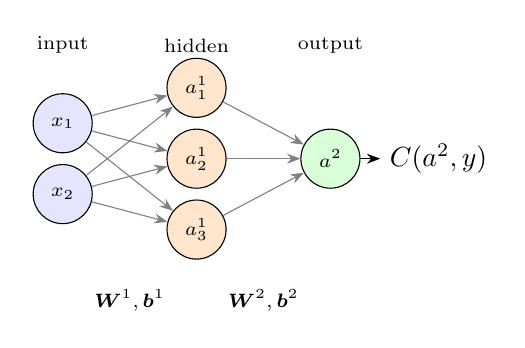
\begin{tikzpicture}[x=1.7cm,y=0.9cm,
    neuron/.style={circle,draw,minimum size=0.75cm,inner sep=0pt,font=\scriptsize},
    >=Stealth]
  \foreach \i in {1,2} \node[neuron,fill=blue!10] (x\i) at (0,-\i-0.5) {$x_{\i}$};
  \foreach \j in {1,2,3} \node[neuron,fill=orange!20] (h\j) at (1,-\j) {$a^1_{\j}$};
  \node[neuron,fill=green!15] (o) at (2,-2) {$a^2$};
  \node[right=0.25cm of o] (C) {$C(a^2,y)$};
  \foreach \i in {1,2} \foreach \j in {1,2,3} \draw[->,gray] (x\i) -- (h\j);
  \foreach \j in {1,2,3} \draw[->,gray] (h\j) -- (o);
  \draw[->] (o) -- (C);
  \node[font=\scriptsize] at (0.5,-4.0) {$\bm{W}^1,\bm{b}^1$};
  \node[font=\scriptsize] at (1.5,-4.0) {$\bm{W}^2,\bm{b}^2$};
  \node[font=\scriptsize] at (0,-0.4) {input};
  \node[font=\scriptsize] at (1,-0.4) {hidden};
  \node[font=\scriptsize] at (2,-0.4) {output};
\end{tikzpicture}
\end{column}
\begin{column}{0.53\textwidth}
One sample $\bm{x}$, layers $l=1,\dots,L$, $\bm{a}^{0}=\bm{x}$:
\[
  \boxed{\;\bm{z}^{l}=\bm{W}^{l}\bm{a}^{l-1}+\bm{b}^{l},\qquad
  \bm{a}^{l}=f(\bm{z}^{l})\;}
\]
\small
\begin{itemize}
  \item $\bm{W}^{l}$ has shape (nodes out, nodes in)
  \item $f$ acts element by element; the last layer has its own
        \emph{output} activation $f_{L}$
  \item the cost $C$ compares the output $\bm{a}^{L}$ with the target
        $\bm{y}$
\end{itemize}
\vspace{4pt}
\footnotesize In code with many samples we stack them as rows,
$\bm{Z}^{l}=\bm{A}^{l-1}\bm{W}^{l}+\bm{b}^{l}$, so $\bm{W}^{l}$ is stored
as (in, out): the same equations, transposed.
\end{column}
\end{columns}
\end{frame}

\begin{frame}{Backpropagation: the chain rule, organised}
\begin{columns}[T]
\begin{column}{0.42\textwidth}
\centering
\begin{tikzpicture}[x=2.0cm,y=0.75cm,>=Stealth,
    v/.style={circle,draw,minimum size=0.6cm,inner sep=0pt,font=\scriptsize}]
  \node[v] (p0) at (0,0) {};
  \node[v,fill=blue!10,thick] (p1) at (0,-1) {$i$};
  \node[v] (p2) at (0,-2) {};
  \node[v] (q0) at (1,0) {};
  \node[v,fill=orange!25,thick] (q1) at (1,-1) {$j$};
  \node[v] (q2) at (1,-2) {};
  \foreach \r in {0,1,2} \node[v,fill=green!15] (s\r) at (2,-\r) {$k$};
  \foreach \a in {0,1,2} \foreach \b in {0,1,2} {
    \draw[->,gray!35] (p\a)--(q\b);
    \draw[->,gray!35] (q\a)--(s\b);}
  \draw[->,thick,blue!60!black] (p1)--(q1)
    node[midway,below,font=\scriptsize]{$w^{l}_{ji}$};
  \foreach \r in {0,1,2} \draw[->,thick,structure.fg] (q1)--(s\r);
  \node[font=\scriptsize,structure.fg,fill=white,inner sep=1pt] at (1.5,-1.5) {$w^{l+1}_{kj}$};
  \node[font=\scriptsize] at (0,0.8) {layer $l-1$};
  \node[font=\scriptsize] at (1,0.8) {layer $l$};
  \node[font=\scriptsize] at (2,0.8) {layer $l+1$};
  \node[font=\scriptsize] at (0,-2.75) {$a^{l-1}_{i}$};
  \node[font=\scriptsize] at (1,-2.75) {$z^{l}_{j}$, $\delta^{l}_{j}$};
  \node[font=\scriptsize] at (2,-2.75) {$\delta^{l+1}_{k}$};
\end{tikzpicture}
\end{column}
\begin{column}{0.56\textwidth}
\small
Node $j$ in layer $l$, one sample:
\[
  z^{l}_{j}=\sum_{i}w^{l}_{ji}\,a^{l-1}_{i}+b^{l}_{j},\qquad
  a^{l}_{j}=f(z^{l}_{j})
\]
The \emph{error} of node $j$ is
$\displaystyle\delta^{l}_{j}=\frac{\partial C}{\partial z^{l}_{j}}$.
\begin{boardbox}{Chain rule}
Chain rule: $\delta^{L}_{j}$, then $\delta^{l}_{j}$ from all the
$\delta^{l+1}_{k}$, then $\partial C/\partial w^{l}_{ji}$ and
$\partial C/\partial b^{l}_{j}$. 
\end{boardbox}
\end{column}
\end{columns}
\pause
\vspace{-2pt}
\begin{block}{Result}
\vspace{-8pt}
\[
  \delta^{L}_{j}=f_{L}'(z^{L}_{j})\,\frac{\partial C}{\partial a^{L}_{j}},\qquad
  \delta^{l}_{j}=\Bigl(\sum_{k}w^{l+1}_{kj}\,\delta^{l+1}_{k}\Bigr)f'(z^{l}_{j}),\qquad
  \frac{\partial C}{\partial w^{l}_{ji}}=\delta^{l}_{j}\,a^{l-1}_{i},\qquad
  \frac{\partial C}{\partial b^{l}_{j}}=\delta^{l}_{j}
\]
\end{block}
\vspace{-4pt}
\footnotesize
\begin{itemize}
  \item Start at the output, go \emph{backwards}: each $\delta^{l}$ reuses
        $\delta^{l+1}$.
  \item Node $j$ feeds \emph{every} node $k$ of layer $l+1$, so its error
        comes back along every edge: the sum over $k$.
  \item Weight gradient $=$ error at the end of the edge $\times$ signal at
        its start.  The error picks up a factor $w\,f'$ in every layer.
\end{itemize}
\end{frame}

\begin{frame}{The general case: a batch of samples}
\begin{columns}[T]
\begin{column}{0.44\textwidth}
\small
As in code: stack the $n$ samples as \textbf{rows}, $\bm{A}^{0}=\bm{X}$ of
shape $(n,n_{0})$, and store $\bm{W}^{l}$ as (in, out), shape
$(n_{l-1},n_{l})$:
\[
  \bm{Z}^{l}=\bm{A}^{l-1}\bm{W}^{l}+\bm{b}^{l},\qquad
  \bm{A}^{l}=f(\bm{Z}^{l}),
\]
with $\bm{b}^{l}$ added to every row.  The cost is the mean over the batch,
$C=\frac1n\sum_{s}C_{s}$, and the errors form a matrix with one row per
sample $s$:
\[
  \Delta^{l}_{sj}=\frac{\partial C}{\partial Z^{l}_{sj}}.
\]
\footnotesize The $\frac1n$ of the mean sits in
$\partial C/\partial\bm{A}^{L}$; $\circ$ is the element-wise product.
\end{column}
\begin{column}{0.54\textwidth}
\begin{block}{Backpropagation for a batch}
\vspace{-6pt}
\begin{align*}
  \bm{\Delta}^{L}&=f_{L}'(\bm{Z}^{L})\circ\frac{\partial C}{\partial\bm{A}^{L}}\\
  \bm{\Delta}^{l}&=\bigl(\bm{\Delta}^{l+1}(\bm{W}^{l+1})^{T}\bigr)\circ f'(\bm{Z}^{l})\\
  \frac{\partial C}{\partial\bm{W}^{l}}&=(\bm{A}^{l-1})^{T}\bm{\Delta}^{l}\\
  \frac{\partial C}{\partial\bm{b}^{l}}&=\textstyle\sum_{s}\bm{\Delta}^{l}_{s,:}
     \quad\text{(sum of the rows)}
\end{align*}
\end{block}
\footnotesize
\begin{itemize}
  \item The one-sample equations, transposed: samples are rows.
  \item Shapes: $\bm{\Delta}^{l}$ is $(n,n_{l})$, and
        $(\bm{A}^{l-1})^{T}\bm{\Delta}^{l}$ is $(n_{l-1},n_{l})$, the shape
        of $\bm{W}^{l}$.
  \item The matrix product sums over the samples: the gradient of the
        whole batch in one operation per layer.
\end{itemize}
\end{column}
\end{columns}
\end{frame}

\begin{quickq}[why not start at zero?]
\begin{columns}[T]
\begin{column}{0.5\textwidth}
\question{A network starts with \emph{all} weights and biases equal to
zero.  Look at the equations: which gradients are non-zero after the
first backward pass?  What happens after that?}
\vspace{4pt}
\begin{align*}
  \bm{\delta}^{L}&=f_{L}'(\bm{z}^{L})\circ\frac{\partial C}{\partial\bm{a}^{L}}\\
  \bm{\delta}^{l}&=\bigl((\bm{W}^{l+1})^{T}\bm{\delta}^{l+1}\bigr)\circ f'(\bm{z}^{l})\\
  \frac{\partial C}{\partial\bm{b}^{l}}&=\bm{\delta}^{l},\qquad
  \frac{\partial C}{\partial\bm{W}^{l}}=\bm{\delta}^{l}\,(\bm{a}^{l-1})^{T}
\end{align*}
\end{column}
\begin{column}{0.48\textwidth}
\answer{Only the \textbf{output layer}.
\begin{itemize}
  \item $\bm{W}^{l+1}=\bm{0}$ gives $\bm{\delta}^{l}=\bm{0}$ in every
        hidden layer, whatever $f$ is: no hidden weight or bias moves.
  \item Learning has to creep backwards from the output, one layer per
        step, and every gradient is a product of near-zero weights.
        Slow to start at best; if $f(0)=0$ the network never leaves
        $\bm{W}=\bm{0}$.
  \item \textbf{Symmetry}: all units in a layer start identical, so they
        get identical gradients and stay copies of each other.  The same
        happens for any equal non-zero start.
\end{itemize}
\textbf{Random weights break the symmetry.}}
\end{column}
\end{columns}
\end{quickq}

%% ====================================================================
%% Part 2: activation functions and cost functions
%% ====================================================================

\section{Activation and cost functions}

\begin{frame}{Hidden activation functions}
\centering
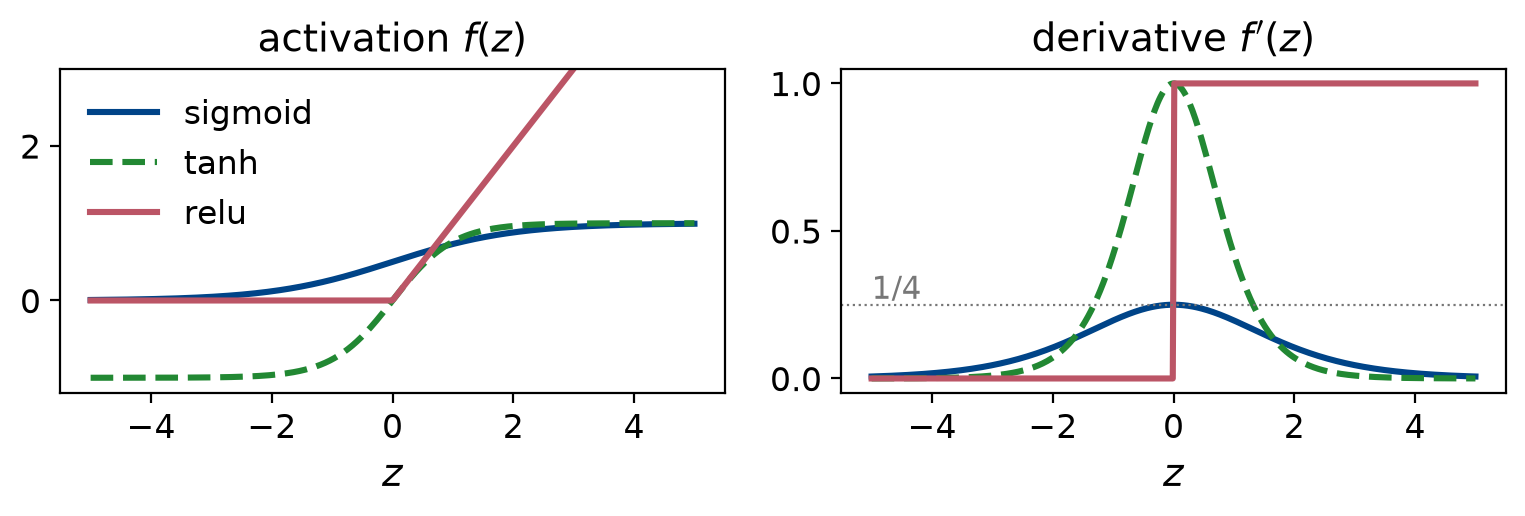
\includegraphics[width=0.78\textwidth]{activations}\par
\vspace{2pt}
\raggedright\small
\begin{columns}[T]
\begin{column}{0.33\textwidth}
\textbf{Sigmoid} $\sigma(z)=\frac{1}{1+e^{-z}}$\\
$\sigma'=\sigma(1-\sigma)\le\frac14$.\\
Flat ($\sigma'\approx0$) for large $|z|$.
\end{column}
\begin{column}{0.33\textwidth}
\textbf{tanh}\\
$\tanh'=1-\tanh^{2}\le1$.\\
Centred at zero; also flat for large $|z|$.
\end{column}
\begin{column}{0.33\textwidth}
\textbf{ReLU} $\max(0,z)$\\
$f'=1$ for $z>0$, $0$ otherwise.  A unit with $z<0$ for all inputs never
learns (``dead'').
\end{column}
\end{columns}
\vspace{4pt}
\begin{block}{What matters}
$f$ must be \textbf{non-linear}: otherwise the whole network is a single
linear map.  For training, $f'$ matters.  Backpropagation multiplies by
$f'$ once per layer, so with $L$ sigmoid layers the $f'$ factors alone
multiply the error by at most $(\tfrac14)^{L}$: the \emph{vanishing
gradient}.  This is why ReLU is the
default in deep networks.
\end{block}
\end{frame}

\begin{frame}{Initialising the weights}
\begin{columns}[T]
\begin{column}{0.5\textwidth}
\small
\textbf{Random}, to break the symmetry.  \textbf{The scale matters.}
$\bm{z}=\bm{W}\bm{a}+\bm{b}$ with $M$ inputs, and independent zero-mean
entries of variance $\sigma_w^{2}$ in $\bm{W}$ and $\sigma_b^{2}$ in
$\bm{b}$:
\[
  \mathbb{E}[\bm{z}\bm{z}^{T}]
  =\mathbb{E}[\bm{W}\bm{a}\bm{a}^{T}\bm{W}^{T}]+\mathbb{E}[\bm{b}\bm{b}^{T}]
  =\bigl(M\sigma_w^{2}\,\overline{a^{2}}+\sigma_b^{2}\bigr)\bm{I}
\]
With $\bm{b}=\bm{0}$, $\operatorname{Var}(z)=M\sigma_w^{2}\,\overline{a^{2}}$, where $\overline{a^{2}}$ is the mean squared \emph{incoming} activation.
For tanh near zero $a\approx z$, so each layer multiplies the variance by $M\sigma_w^{2}$.
\begin{itemize}
  \item $\sigma_w$ too large: $|z|$ large, tanh/sigmoid saturate,
        gradients blow up or die.
  \item $\sigma_w$ too small: the signal shrinks in every layer, and so do
        the gradients.
\end{itemize}
\end{column}
\begin{column}{0.48\textwidth}
\begin{block}{Rule: keep $\operatorname{Var}(z)$ the same in every layer}
\[
  \sigma_w^{2}=\frac{1}{M}\ \text{(tanh)},\qquad
  \sigma_w^{2}=\frac{2}{M}\ \text{(ReLU)}
\]
ReLU sets half of its inputs to zero, so
$\overline{a^{2}}=\frac12\operatorname{Var}(z)$: hence the factor 2 (``He
initialisation'').  Sigmoid: $\sigma'\le\frac14$, so with $1/M$ the
gradients still shrink layer by layer.
\end{block}
\small The right scale depends on the \emph{activation function}, and
it decides whether \emph{gradients} survive the backward pass.
\end{column}
\end{columns}
\end{frame}

\begin{frame}{The wrong scale breaks a deep network before training starts}
\small A deep network: 256 inputs $\to$ \textbf{10 hidden layers, each with
256 tanh units} $\to$ one linear output unit, no biases.  Input: 500 random
Gaussian vectors; targets: random numbers; cost
$C=\tfrac12\,\overline{(a^{L}-y)^{2}}$.
Nothing is trained: one forward and one backward pass.\par
\centering
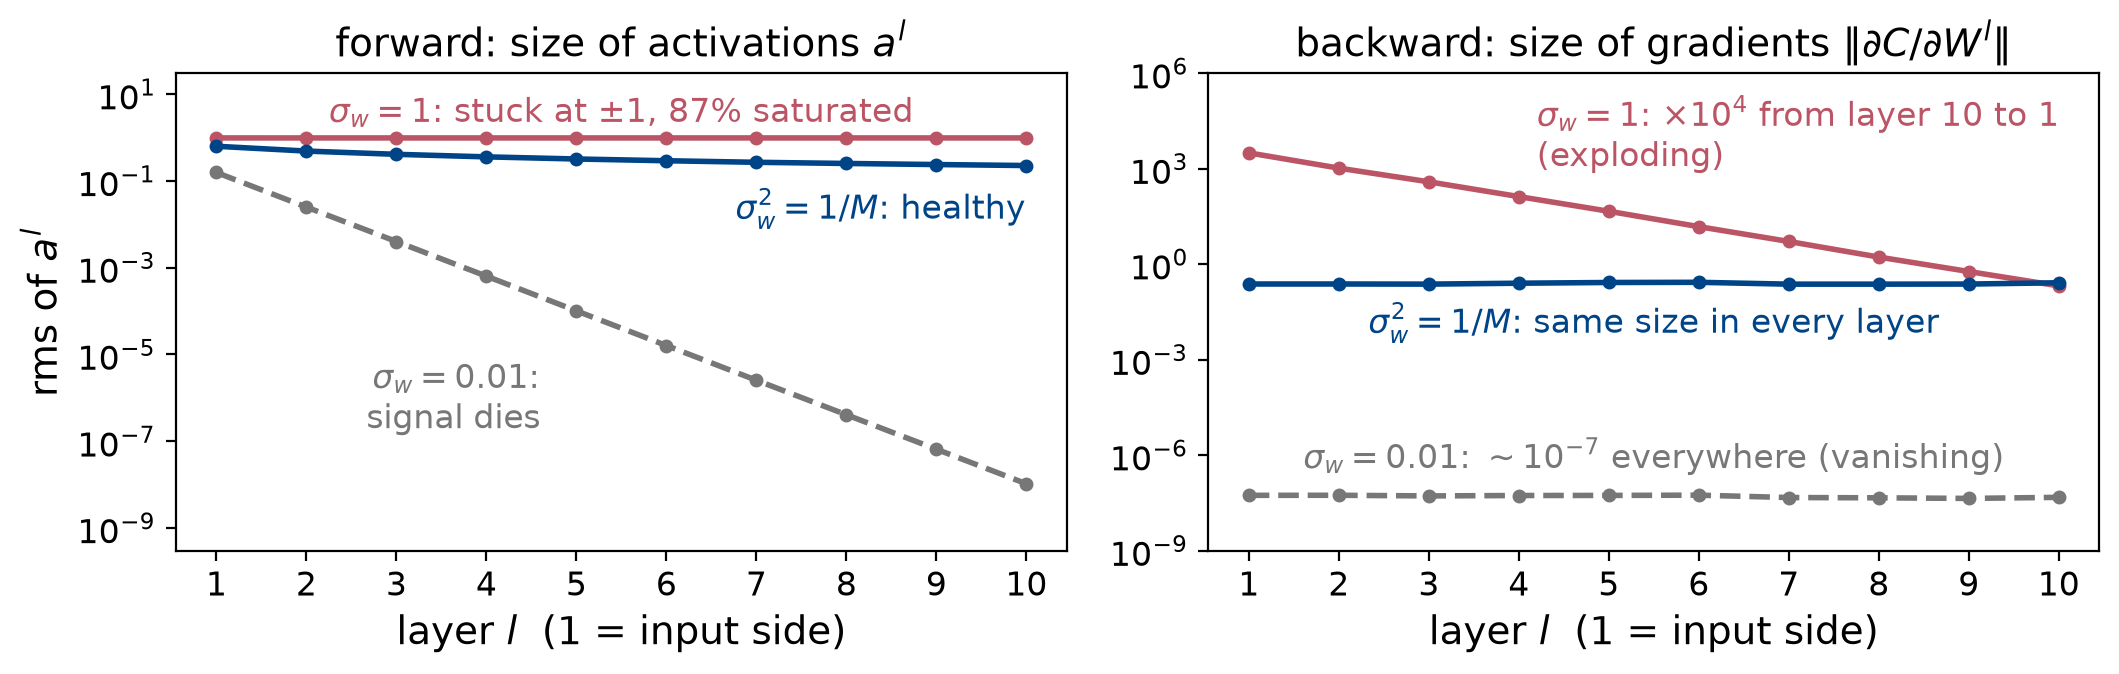
\includegraphics[width=\textwidth]{init}\par
\raggedright
\begin{itemize}
  \item \textcolor[HTML]{BB5566}{\textbf{Too large:}} saturated units and
        exploding gradients.
  \item \textcolor[HTML]{777777}{\textbf{Too small:}} the signal dies and the
        gradients vanish.
  \item Either way, gradient descent cannot train the network.
  \item \textcolor[HTML]{004488}{\textbf{$\sigma_w^{2}=1/M$:}} signal and
        gradients keep their size through all 10 layers.
\end{itemize}
\end{frame}

\begin{frame}{The right scale depends on the activation function}
\begin{columns}[T]
\begin{column}{0.46\textwidth}
\small
The same network with \textbf{ReLU} instead of tanh, initialised with the
rule that worked for tanh, $\sigma_w^{2}=1/M$:
\begin{itemize}
  \item The signal shrinks by $\sqrt2$ in \emph{every} layer: $1/23$ of its
        size after 10 layers, $\sim10^{-7}$ after 50.
  \item No error message.  The network just trains slowly, or not at all.
\end{itemize}
\vspace{4pt}
\textbf{Why:} ReLU sets half of its inputs to zero, so it passes on only
half the variance.  He initialisation, $\sigma_w^{2}=2/M$, makes up for it.
\vspace{6pt}
\begin{block}{Take-away}
An initialisation rule belongs to an activation function.  Change the
activation, and check the scale again.
\end{block}
\end{column}
\begin{column}{0.52\textwidth}
\centering
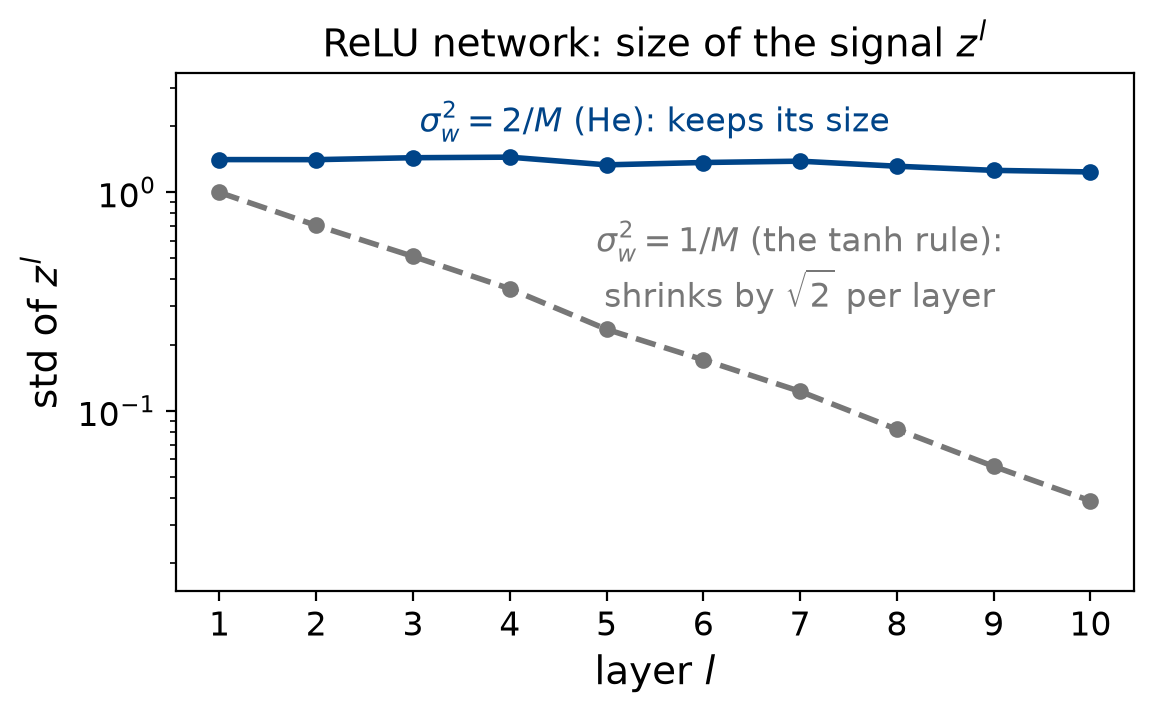
\includegraphics[width=\textwidth]{init_relu}
\end{column}
\end{columns}
\end{frame}

\begin{frame}{Output activation and cost function come in pairs}
\begin{center}
\setlength{\tabcolsep}{6pt}
\begin{tabular}{@{}llll@{}}
\toprule
Task & Output activation & Cost (one sample) & $\bm{\delta}^{L}$\\
\midrule
regression, $y\in\mathbb{R}$ & linear, $a=z$ & $\tfrac12(a-y)^{2}$ & \uncover<2->{$a-y$}\\[2pt]
binary, $y\in\{0,1\}$ & sigmoid, $a=\sigma(z)$ & $-y\ln a-(1-y)\ln(1-a)$ & \uncover<2->{$a-y$}\\[2pt]
$K$ classes, $\bm{y}$ one-hot & softmax, $a_k=\frac{e^{z_k}}{\sum_le^{z_l}}$ & $-\sum_ky_k\ln a_k$ & \uncover<2->{$\bm{a}-\bm{y}$}\\
\bottomrule
\end{tabular}
\end{center}
\begin{columns}[T]
\begin{column}{0.48\textwidth}
\small
\begin{itemize}
  \item The \textbf{output activation} gives the right \emph{range}: any
        real number, a probability, or $K$ probabilities that sum to one.
  \item The \textbf{cost} matches it: each is the negative log-likelihood of
        a Gaussian, Bernoulli or categorical distribution.
\end{itemize}
\vspace{4pt}
\uncover<2->{\footnotesize Softmax is not element-wise: there, $f'$ is the
Jacobian $\partial a_k/\partial z_j$, but the same cancellation happens.}
\end{column}
\begin{column}{0.5\textwidth}
\small
For these pairs, $\delta^{L}=f_{L}'(z^{L})\,\partial C/\partial a^{L}$.
What happens to $f_{L}'$?
\pause
\begin{block}{$f_L'$ cancels}
For all three pairs, $f_{L}'$ \emph{cancels} against
$\partial C/\partial a$.  Sigmoid: $\sigma'=a(1-a)$ and
$\frac{\partial C}{\partial a}=\frac{a-y}{a(1-a)}$, so
\[
  \boxed{\;\bm{\delta}^{L}=\bm{a}^{L}-\bm{y}\;}\quad
  \text{prediction minus target.}
\]
\end{block}
\end{column}
\end{columns}
\end{frame}

\begin{frame}{What goes wrong with a mismatched pair: sigmoid $+$ squared error}
\begin{columns}[T,onlytextwidth]
\begin{column}{0.46\textwidth}
\small
Sigmoid output $a=\sigma(z)$, target $y=1$:
\vspace{-6pt}
\begin{alignat*}{2}
  &\text{cross entropy:}\quad &\delta^{L}_{\mathrm{CE}}&=a-1\\
  &\text{squared error:}\quad &\delta^{L}_{\mathrm{SE}}&=(a-1)\,
     \textcolor[HTML]{BB5566}{\underbrace{a(1-a)}_{\sigma'(z)}}
\end{alignat*}
\end{column}
\begin{column}{0.5\textwidth}
\small
Here $\sigma'$ does \emph{not} cancel, and $\sigma'\to0$ as $a\to0$.\\
At $z=-5$: $\delta^{L}_{\mathrm{SE}}$ is \textbf{150$\times$ smaller}
than $\delta^{L}_{\mathrm{CE}}$.
\vspace{-4pt}
\begin{block}{}
Squared error: the more confidently wrong, the \emph{less} it learns.
\end{block}
\end{column}
\end{columns}
\vspace{-2pt}
\centering
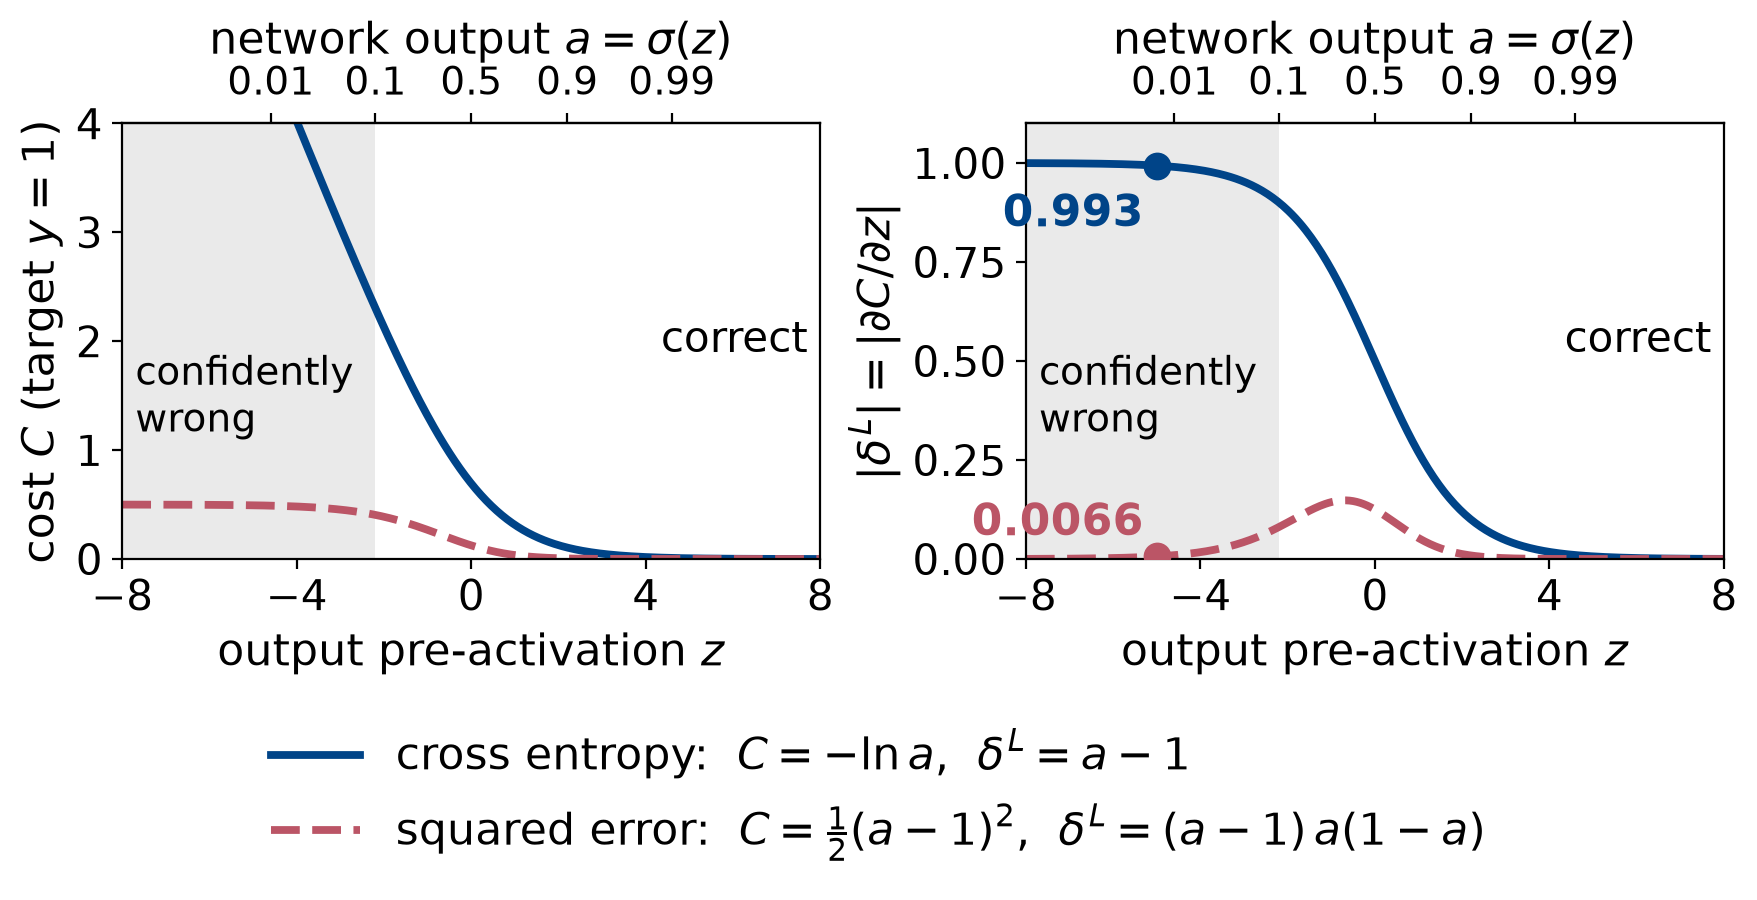
\includegraphics[width=0.76\textwidth]{delta_heads}
\end{frame}

\begin{quickq}[which image trains the network?]
\begin{columns}[c]
\begin{column}{0.44\textwidth}
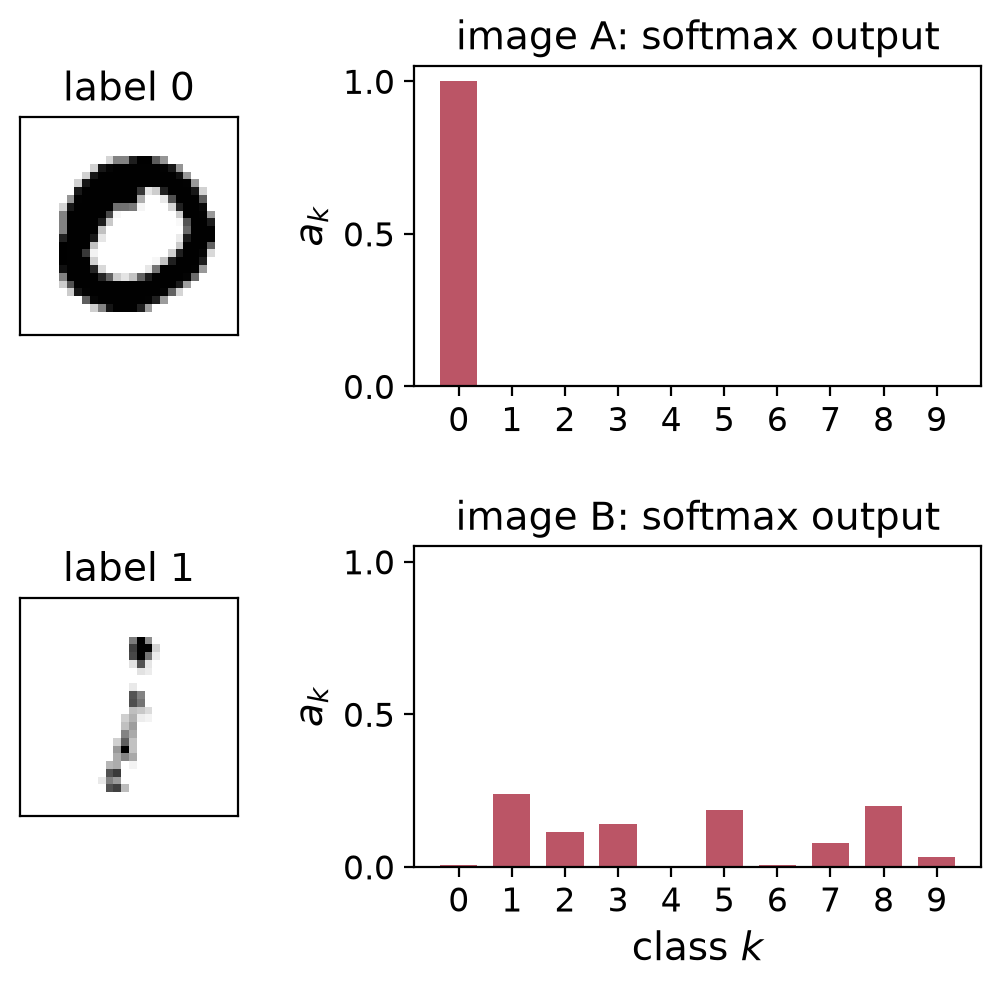
\includegraphics[width=\textwidth]{mnist_question}
\end{column}
\begin{column}{0.54\textwidth}
\question{A network trained on handwritten digits (softmax $+$ cross
entropy) sees images A and B.  The error
$\bm{\delta}^{L}=\bm{a}^{L}-\bm{y}$ has one component per class
$0,\dots,9$; $\bm{y}$ is the one-hot label.  Which image changes the
weights more?}
\answer{A, label 0: $\bm{a}\approx\bm{y}=(1,0,\dots,0)$, so
$\bm{\delta}^{L}\approx\bm{0}$: nothing to learn.\\[2pt]
B, label 1: $\bm{y}=(0,1,0,\dots,0)$.
\begin{itemize}
  \item $\delta_{1}=a_{1}-1=0.24-1=-0.76$: the only negative component.
  \item Every other $\delta_{k}=a_{k}-0=a_{k}>0$.
\end{itemize}
Raise the score of class 1, lower the rest.  The network learns from
what it gets wrong or is unsure about.}
\end{column}
\end{columns}
\end{quickq}

%% ====================================================================
%% Part 3: universal approximation
%% ====================================================================

\section{Universal approximation}

\begin{frame}{The universal approximation theorem}
\begin{block}{In words}
A network with \textbf{one hidden layer} and a \textbf{non-linear}
(non-polynomial) activation can approximate \textbf{any continuous
function} on a bounded domain \textbf{as accurately as we want}, if the
hidden layer is wide enough.
\end{block}
\vspace{6pt}
\begin{columns}[T]
\begin{column}{0.46\textwidth}
\begin{block}{What it says}
\begin{itemize}
  \item A network \emph{can} represent the function we are after.
  \item The non-linearity is essential.
\end{itemize}
\end{block}
\end{column}
\begin{column}{0.5\textwidth}
\begin{block}{What it does \emph{not} say}
\begin{itemize}
  \item \emph{How many} units are needed.
  \item Whether training \emph{finds} the weights.
  \item How well it generalises to new data.
\end{itemize}
\end{block}
\end{column}
\end{columns}
\vspace{4pt}
\small Why deep networks, then?  For many functions, depth does the same
job with far fewer units.
\end{frame}

\begin{frame}{Why it works, in one dimension: ReLU units are kinks}
\begin{columns}[T]
\begin{column}{0.5\textwidth}
\small
One ReLU unit $v\,\mathrm{ReLU}(wx+b)$ is zero, then a straight line: one
\emph{kink}, at $x=-b/w$.  Three units make a ``hat'':
\[
  \mathrm{ReLU}(x)-2\,\mathrm{ReLU}(x-1)+\mathrm{ReLU}(x-2)
\]
\centering
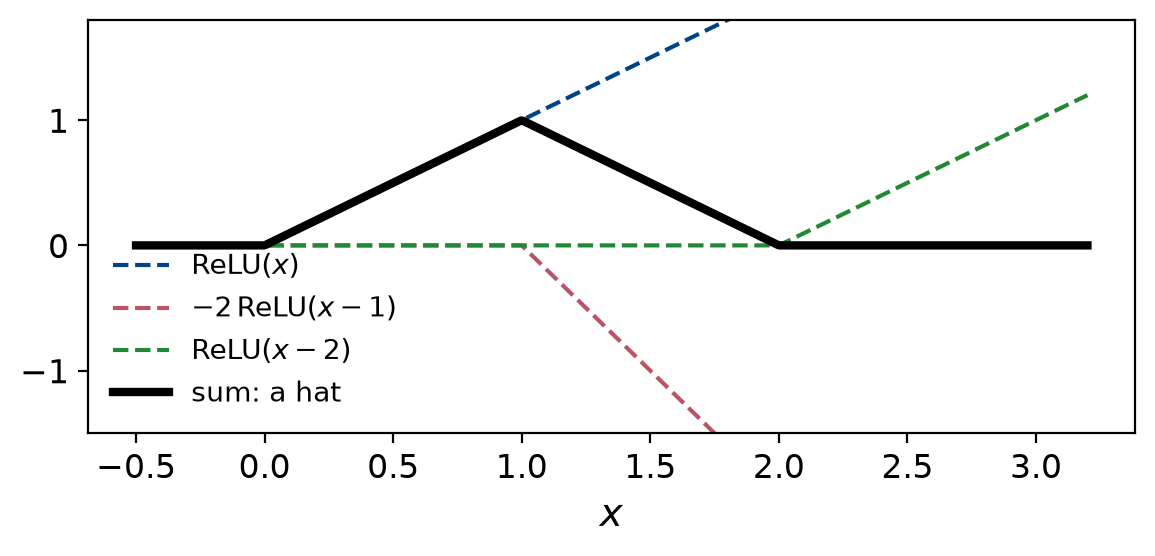
\includegraphics[width=\textwidth]{relu_hat}\par
\raggedright
\pause
\textbf{Any function $F$:} one hat of height $F(x_i)$ at each point $x_i$.
Their sum connects the dots $(x_i,F(x_i))$ with straight lines.  More
points, smaller error.
\pause
\end{column}
\begin{column}{0.48\textwidth}
\onslide<3->{
\centering
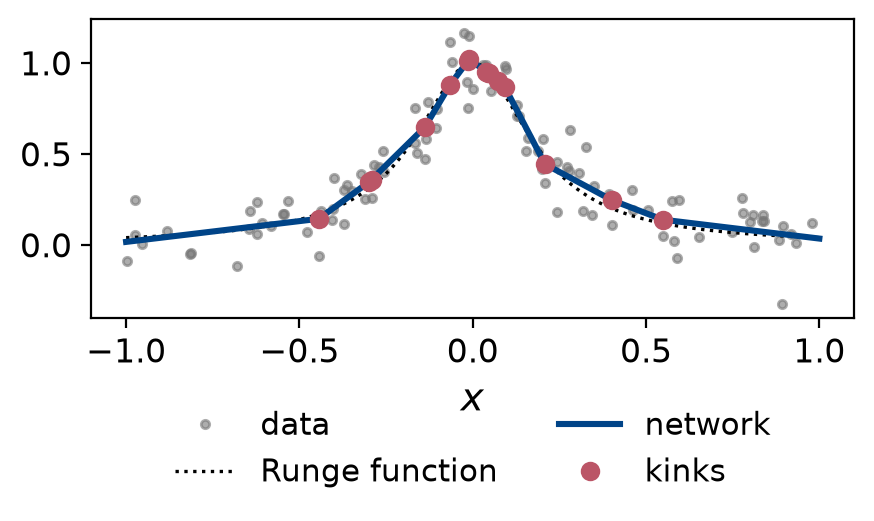
\includegraphics[width=\textwidth]{runge_kinks}\par
\raggedright\small Training finds this by itself: a network with 50 ReLU
units fitted to noisy data from the Runge function.  The output is
piecewise linear, and the kinks (red) sit where the function bends.}
\end{column}
\end{columns}
\end{frame}

\begin{frame}{Universal approximation: the precise statements}
\begin{columns}[T]
\begin{column}{0.52\textwidth}
\begin{block}{The theorem (Leshno et al.\ 1993)}
\small
Let $f$ be continuous.  One-hidden-layer networks
\[
  G(\bm{x})=\sum_{j=1}^{N}v_j\,f(\bm{w}_j^{T}\bm{x}+b_j)
\]
can approximate every continuous $F$ on a compact $K\subset\mathbb{R}^{d}$
to any accuracy $\epsilon$,
$\sup_{\bm{x}\in K}|F(\bm{x})-G(\bm{x})|<\epsilon$,
\textbf{if and only if $f$ is not a polynomial}.
\end{block}
\footnotesize
\begin{itemize}
  \item Earlier versions: Cybenko 1989 (sigmoids), Hornik 1991 (any
        bounded, non-constant $f$; also in mean square).
  \item Why not a polynomial: if $f$ has degree $p$, so has $G$, for
        \emph{any} $N$.
\end{itemize}
\end{column}
\begin{column}{0.46\textwidth}
\begin{block}{How many units?}
\footnotesize
\begin{itemize}
  \item \textbf{1D, ReLU:} the hat construction is the piecewise-linear
        interpolant.  For $|F'|\le L$ on $[a,b]$:
        $\sup_x|F-G|\le\dfrac{L(b-a)}{2N}$.
  \item \textbf{$d$ dimensions, grid-like constructions:} error
        $\sim N^{-1/d}$, so $\sim\epsilon^{-d}$ units: the curse of
        dimensionality.
  \item \textbf{Smooth enough $F$} (Barron 1993): if
        $C_F=\int|\bm{\omega}|\,|\hat F(\bm{\omega})|\,d\bm{\omega}<\infty$,
        a sigmoid network reaches mean-square error
        $\lesssim C_F^{2}/N$, \emph{independent of $d$}.
  \item \textbf{Depth:} some functions need exponentially many units in
        one hidden layer, but only polynomially many in a deep network
        (Telgarsky 2016).
\end{itemize}
\end{block}
\footnotesize Still nothing about whether gradient descent \emph{finds}
these weights.
\end{column}
\end{columns}
\end{frame}

%% ====================================================================
%% Part 4: differential equations
%% ====================================================================

\section{Neural networks for differential equations}

\begin{frame}{From fitting data to solving equations}
\small
Universal approximation: a network $N(x)$ can represent any function.  So
it can also represent the \emph{solution} of a differential equation.
But what do we train it on?
\vspace{0pt}
\begin{columns}[T]
\begin{column}{0.48\textwidth}
\begin{block}{So far: fit data}
Targets $y_i$ are given.  Cost: how far the output is from them,
\[
  C=\frac1n\sum_i\bigl(N(x_i)-y_i\bigr)^{2}
\]
\end{block}
\end{column}
\begin{column}{0.48\textwidth}
\begin{block}{Now: solve $g'=-\alpha g$}
No targets: the solution is unknown.  Cost: how badly the output violates
the \emph{equation},
\[
  C=\frac1n\sum_i\bigl(N'(x_i)+\alpha N(x_i)\bigr)^{2}
\]
\end{block}
\end{column}
\end{columns}
Network, backpropagation and optimiser stay the same; only the cost
changes.  This is a \textbf{physics-informed neural network} (PINN).
\begin{block}{Take-aways}
\begin{enumerate}\setlength{\itemsep}{0pt}
  \item Why the activation function matters: we need $N'$ and $N''$
  \item Boundary conditions: built in (hard) or as penalties (soft)
  \item Against standard methods: Euler, Runge--Kutta, finite differences
  \item Equation $+$ data: inverse problems, unknown parameters
\end{enumerate}
\end{block}
\end{frame}

\begin{frame}{Learning the equation: the residual is the cost}
\begin{columns}[T]
\begin{column}{0.52\textwidth}
\small
\textbf{Problem:} $g'(x)+\alpha g(x)=0$, $g(0)=g_0$.  The network learns
the \emph{equation}: the cost measures how badly its output violates
it.\\[2pt]
\textbf{Three ingredients:}
\begin{enumerate}
  \item A \textbf{trial solution} that satisfies the conditions for
        \emph{any} network $N$: $g_t(x)=h(x)+B(x)\,N(x)$, where $h$
        satisfies the conditions and $B=0$ where they are imposed.
  \item The \textbf{residual}: the left-hand side for $g_t$,
        $r(x)=g_t'(x)+\alpha\,g_t(x)$; zero for the exact solution.
  \item The \textbf{cost}: the mean squared residual at points $x_i$ we
        choose ourselves (\emph{collocation points}),
        \[
          C=\frac1n\sum_{i=1}^{n}r(x_i)^{2}.
        \]
\end{enumerate}
\end{column}
\begin{column}{0.46\textwidth}
\begin{block}{What is new}
The residual contains $g_t'$, so we need $\partial N/\partial x$: a
derivative with respect to the \emph{input}, not the weights.  It is just as
easy to compute as the derivatives with respect to the weights.
\end{block}
\begin{block}{What is not new}
Network, optimiser and backpropagation for the weights.  It is regression
with ``target'' $r=0$.
\end{block}
\end{column}
\end{columns}
\end{frame}

\begin{frame}{Example: exponential decay}
\begin{columns}[T]
\begin{column}{0.5\textwidth}
\small
$g'+\alpha g=0$, $g(0)=g_0$, with $\alpha=2$, $g_0=10$.  Exact solution:
$g=g_0e^{-\alpha x}$.
\begin{boardbox}{Exponential decay}
Build $g_t$, compute $g_t'$, write the residual and the cost.
\end{boardbox}
\pause
\[
  g_t=g_0+x\,N(x),\qquad
  r=\underbrace{N+x\,N'}_{g_t'}+\alpha\,(g_0+x\,N)
\]
$g_t(0)=g_0$ whatever the network does.
\end{column}
\begin{column}{0.48\textwidth}
\onslide<2->{
\centering
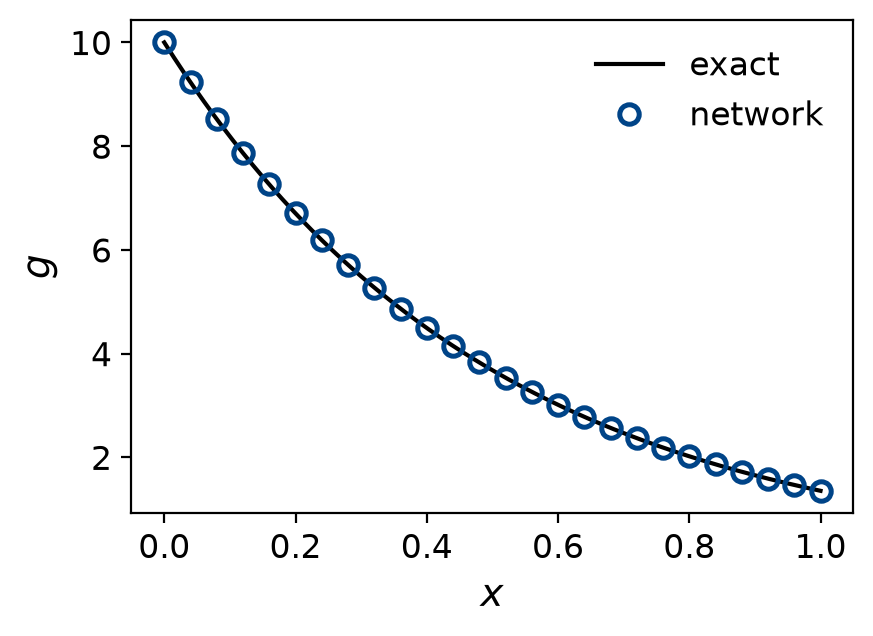
\includegraphics[width=0.9\textwidth]{ode_decay}\par
\raggedright\small Two hidden layers of 40 tanh units, 50 collocation
points: max error $3\times10^{-3}$.}
\end{column}
\end{columns}
\end{frame}

\begin{frame}{The activation function matters even more now}
\begin{columns}[T]
\begin{column}{0.54\textwidth}
\small
{\centering
\setlength{\tabcolsep}{6pt}
\begin{tabular}{@{}ccc@{}}
Poisson & diffusion & wave\\[2pt]
$g''(x)+f(x)=0$ & $\partial_{t}g-\partial_{x}^{2}g=0$ &
$\partial_{t}^{2}g-c^{2}\,\partial_{x}^{2}g=0$
\end{tabular}\par}
\vspace{6pt}
All three contain a \emph{second} derivative, so we need $N''(x)$.
\begin{boardbox}{Second derivatives}
Differentiate a one-hidden-layer network
$N(x)=\sum_jv_j\,f(w_jx+b_j)+c$ twice with respect to $x$.
\end{boardbox}
\pause
\[
  N''(x)=\sum_jv_j\,w_j^{2}\,f''(w_jx+b_j)
\]
\end{column}
\begin{column}{0.44\textwidth}
\onslide<2->{
\begin{block}{ReLU: $f''=0$, so $N''=0$}
A ReLU network is piecewise linear: \emph{no curvature}, for any weights.
It cannot solve $g''+f=0$.
\end{block}
\small
$\max|N''|$ of a randomly initialised network:\\[3pt]
\begin{tabular}{@{}lr@{}}
\toprule
tanh & $2.9$\\
GELU & $1.2$\\
sigmoid & $0.06$\\
ReLU & $\mathbf{0}$\\
\bottomrule
\end{tabular}\\[4pt]
\textbf{We use tanh:} smooth, and $f'=1-f^{2}$, $f''=-2ff'$ are cheap.}
\end{column}
\end{columns}
\end{frame}

\begin{frame}{Boundary conditions built into the trial solution}
\begin{columns}[T]
\begin{column}{0.5\textwidth}
\small
Recipe: $g_t=h(x)+B(x)\,N(x)$, where $h$ satisfies the conditions and
$B=0$ wherever a condition is imposed.
\begin{center}
\setlength{\tabcolsep}{4pt}
\begin{tabular}{@{}ll@{}}
\toprule
Conditions & Trial solution $g_t$\\
\midrule
$g(0)=a,\;g(1)=b$ & $a+(b-a)x+x(1-x)\,N$\\
$g(0)=g_0,\;g'(0)=v_0$ & $g_0+v_0x+x^{2}N$\\
\bottomrule
\end{tabular}
\end{center}
\textbf{Check one row:} put $x=0$ and $x=1$ (for the last row, also
differentiate once).  The $N$ term drops out every time.
\end{column}
\begin{column}{0.48\textwidth}
\begin{block}{The good}
The conditions hold \emph{exactly}, for any weights: at the start, and
after every step.  The optimiser only has to solve the equation.
\end{block}
\begin{block}{The bad}
$g_t$ must be designed by hand for every problem. A curved boundary in 2D or
3D: impractical.
\end{block}
\end{column}
\end{columns}
\end{frame}

\begin{frame}{Two test problems, three standard methods}
\begin{columns}[T]
\begin{column}{0.52\textwidth}
\small
\textbf{Logistic growth}:
\[g'-2g(1-g)=0,\qquad g(0)=1.2.\]
\textbf{Poisson}:
\[g''+(3x+x^{2})e^{x}=0,\qquad g(0)=g(1)=0.\]
\textbf{Standard methods} work on a grid with spacing $\Delta t$ (or
$\Delta x$).
\end{column}
\begin{column}{0.46\textwidth}
\small
\begin{itemize}
  \item \textbf{Forward Euler}: follow the slope for one step,
        $g_{n+1}=g_{n}+\Delta t\,g'(t_{n})$.  Error $\propto\Delta t$.
  \item \textbf{RK4} (Runge--Kutta): four slope evaluations per step.
        Error $\propto\Delta t^{4}$.
  \item \textbf{Finite differences (FD)}:
        $g''(x_i)\approx(g_{i+1}-2g_{i}+g_{i-1})/\Delta x^{2}$ turns the
        equation into a linear system.  Error $\propto\Delta x^{2}$.
\end{itemize}
\end{column}
\end{columns}
\vfill
\pause
\setbeamercolor{block title}{bg=structure.fg,fg=white}%
\setbeamercolor{block body}{bg=structure.fg!8}%
\begin{block}{Guess first}
Network or standard method: which is more \emph{accurate}?  Which is
\emph{faster}?
\end{block}
\end{frame}

\begin{frame}{Results against standard methods}
{\centering
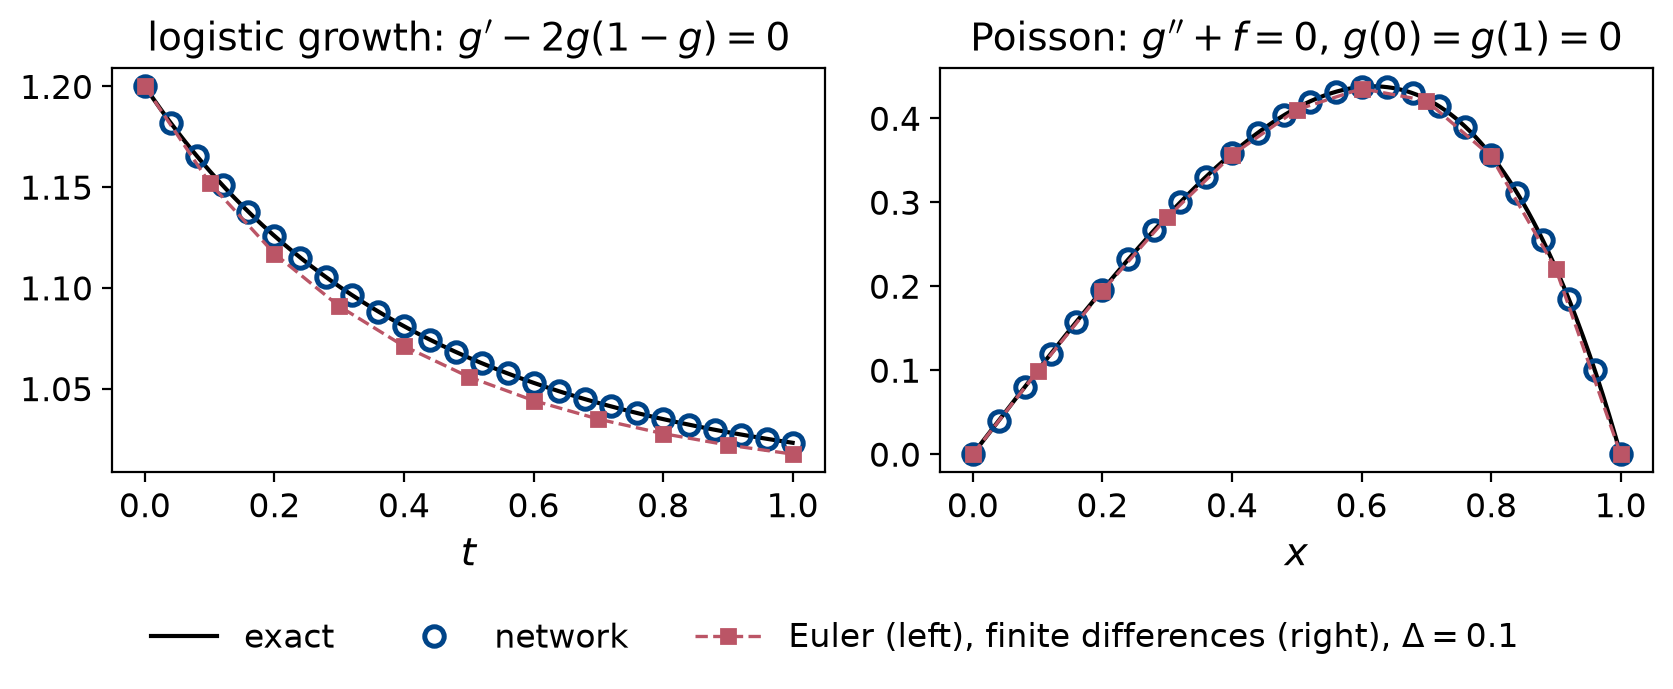
\includegraphics[width=0.72\textwidth]{ode_results}\par}
\vspace{-1.5em}
\begin{columns}[T]
\begin{column}{0.52\textwidth}
\footnotesize
\setlength{\tabcolsep}{4pt}
\begin{tabular}{@{}llrr@{}}
\toprule
& method & max error & time\\
\midrule
logistic & Euler, $\Delta t=0.01$ & $9\times10^{-4}$ & $0.04$ ms\\
         & RK4, $\Delta t=0.01$ & $2\times10^{-10}$ & $0.14$ ms\\
         & network & $1\times10^{-4}$ & $0.5$ s\\
\midrule
Poisson  & FD, $\Delta x=0.01$ & $2\times10^{-5}$ & $0.12$ ms\\
         & network & $1\times10^{-5}$ & $0.6$ s\\
\bottomrule
\end{tabular}\\[2pt]
\scriptsize Network: 4000 training steps of $0.13$--$0.15$ ms each.
Plots use spacing $0.1$, so the grid points are visible.
\end{column}
\begin{column}{0.44\textwidth}
\footnotesize
\begin{block}{Conclusion}
The network beats Euler, but RK4 is far more accurate.  And the network
is thousands of times slower.  For simple equations like these the
standard methods win.
\end{block}
\end{column}
\end{columns}
\end{frame}

\begin{frame}{A partial differential equation: diffusion}
\begin{columns}[T]
\begin{column}{0.46\textwidth}
\[
  \frac{\partial g}{\partial t}-\frac{\partial^{2}g}{\partial x^{2}}=0,\qquad
  \begin{aligned}g(0,t)&=g(1,t)=0,\\ g(x,0)&=\sin\pi x.\end{aligned}
\]
\small The network now has \emph{two inputs}, $N(x,t)$.  Nothing else
changes.
\end{column}
\begin{column}{0.52\textwidth}
Three conditions, one trial solution:
\[
  \boxed{\;g_t=(1-t)\sin\pi x+x(1-x)\,t\,N(x,t)\;}
\]
\small Check: $t=0$ gives $\sin\pi x$; $x=0$ and $x=1$ give $0$.
\end{column}
\end{columns}
\vspace{2pt}
\centering
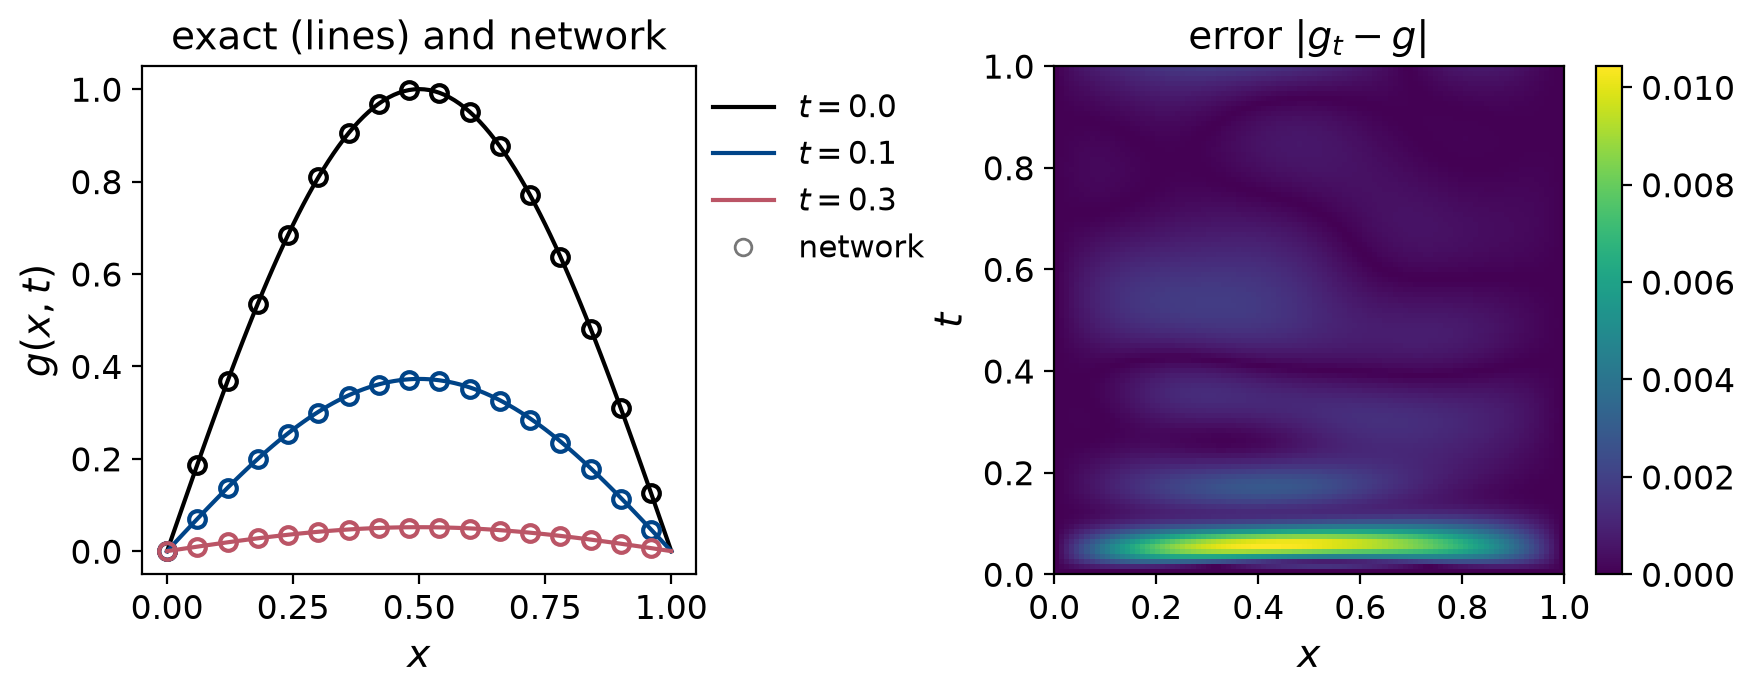
\includegraphics[width=0.68\textwidth]{diffusion}\par
\raggedright\small
Error exactly zero on the three edges (built into $g_t$), largest near
$t=0$ where the solution changes fastest: max $1\times10^{-2}$, after
$1.2$ s of training (800 steps).  Explicit finite differences with
$\Delta x=0.05$: max error $1.5\times10^{-3}$ in $2$ ms.
\end{frame}

\begin{frame}{Soft constraints: conditions as penalties}
\begin{columns}[T]
\begin{column}{0.52\textwidth}
\small
Instead of building $g_t$ by hand: let the network itself be the
solution, $u(x,t)\approx N(x,t)$, and add the conditions to the cost as
penalties:
\[
  L=L_{\mathrm{PDE}}+\lambda\,(L_{\mathrm{IC}}+L_{\mathrm{BC}})
\]
\footnotesize
\vspace{-8pt}
\begin{align*}
  L_{\mathrm{PDE}}&=\tfrac1{n}\textstyle\sum_i(\partial_tN-\partial_x^{2}N)^{2}
     &&\text{inside the domain}\\
  L_{\mathrm{IC}}&=\tfrac1{n}\textstyle\sum_i(N(x_i,0)-\sin\pi x_i)^{2}
     &&\text{at }t=0\\
  L_{\mathrm{BC}}&=\tfrac1{n}\textstyle\sum_i\bigl(N(0,t_i)^{2}+N(1,t_i)^{2}\bigr)
     &&\text{at }x=0,1
\end{align*}
\small
A new condition is just a new term.  $\lambda$ weighs the terms, like the
penalty in Ridge regression.
\end{column}
\begin{column}{0.46\textwidth}
\small
\begin{center}
\begin{tabular}{@{}lcc@{}}
\toprule
& RMSE & error at $t=0$\\
\midrule
hard ($g_t$) & $1.8\times10^{-3}$ & $0$ exactly\\
soft, $\lambda=10$ & $6.5\times10^{-3}$ & $6\times10^{-3}$\\
\bottomrule
\end{tabular}
\end{center}
\begin{block}{Hard or soft?}
\begin{itemize}
  \item If you \emph{can} build a trial solution, do: exact and more
        accurate.
  \item Soft is flexible, but the conditions hold only approximately.
  \item $\lambda$ must be tuned.  Too large, and the optimiser neglects the
        equation.
\end{itemize}
\end{block}
\end{column}
\end{columns}
\end{frame}

\begin{quickq}[a small residual, a wrong answer]
\question{We solve $\partial_tu-\partial_x^{2}u=0$ with the soft cost
$L=L_{\mathrm{PDE}}+\lambda(L_{\mathrm{IC}}+L_{\mathrm{BC}})$, but use a
\textbf{ReLU} network $u=N(x,t)$.  What does training converge to?}
\begin{columns}[T]
\begin{column}{0.5\textwidth}
\answer{\begin{itemize}
  \item ReLU gives $\partial_x^{2}N=0$ at every sample, so
        $L_{\mathrm{PDE}}$ only asks for $\partial_tN=0$.
  \item The network learns $u\approx\sin\pi x$ for all $t$: it never
        diffuses.  Small cost ($6\times10^{-4}$), wrong answer: RMSE
        $0.65$ (vs.\ $1.8\times10^{-3}$).
  \item \textbf{A small residual is not a solution.}  Use smooth
        activations, and check against something you know.
\end{itemize}}
\end{column}
\begin{column}{0.48\textwidth}
\centering
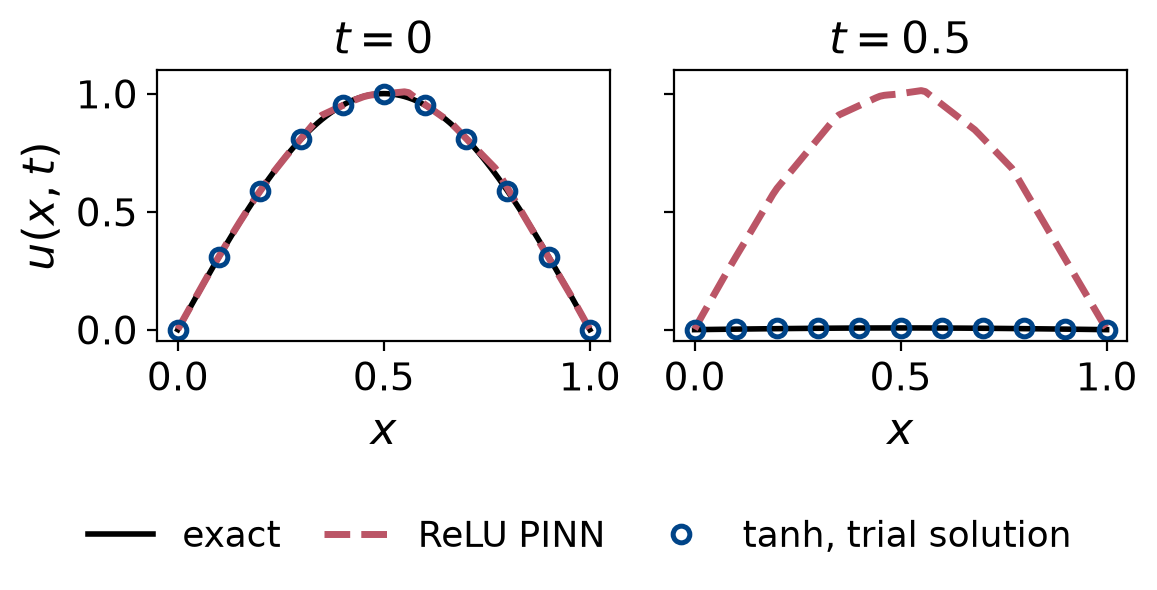
\includegraphics[width=\textwidth]{relu_pinn}
\end{column}
\end{columns}
\end{quickq}

\begin{frame}{Inverse problems: find the unknown parameters of the equation from data}
\begin{columns}[T]
\begin{column}{0.57\textwidth}
\small
$\partial_tu-D\,\partial_x^{2}u=0$ with \textbf{$D$ unknown}.  No initial or
boundary conditions, only $40$ noisy measurements $y_i$.  Treat $D$ as one
more trainable parameter, and fit the equation and the data together:
\[
  L(N,D)=\tfrac1n\textstyle\sum_j\bigl(\partial_tN-D\,\partial_x^{2}N\bigr)^{2}_j
  +\lambda\tfrac1{40}\textstyle\sum_i\bigl(N(x_i,t_i)-y_i\bigr)^{2}
\]
\end{column}
\begin{column}{0.41\textwidth}
\small
A standard solver needs $D$ to run; here the network finds $D$ and the
solution $u$ in one training run.\\[4pt]
True $D=0.5$.  Three different starting guesses all give $D\approx0.51$.
\textbf{But} with five times more noise: $D=0.69$.  A recovered parameter
needs an error bar.
\end{column}
\end{columns}
\vspace{2pt}
\centering
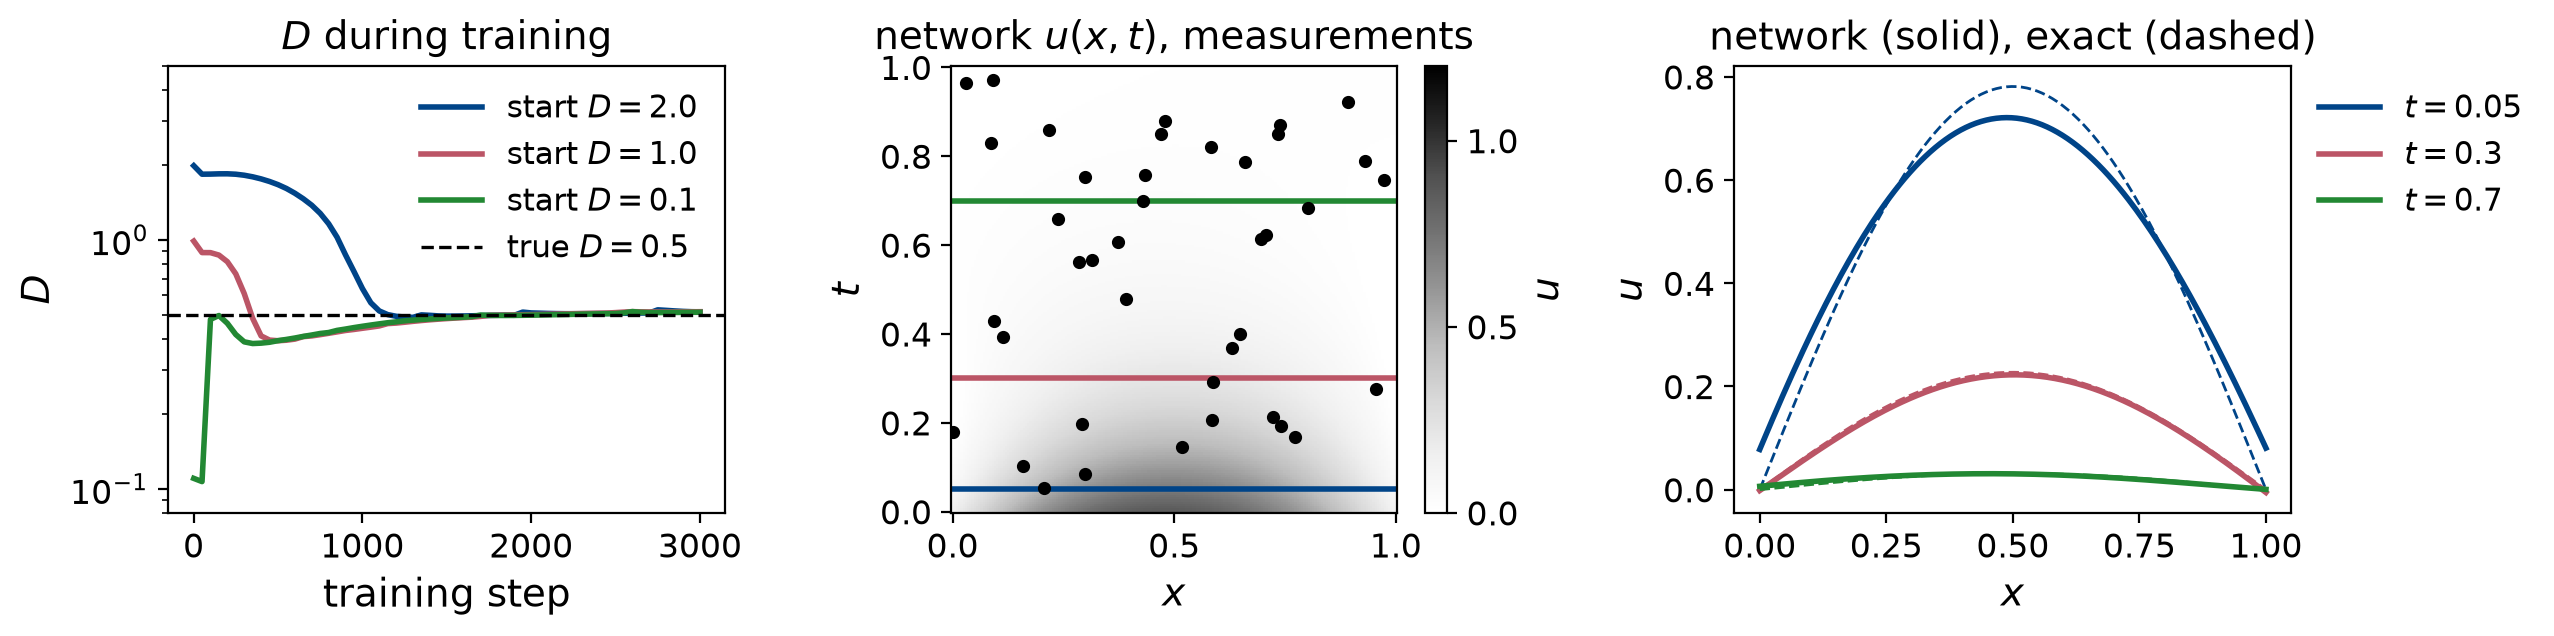
\includegraphics[width=\textwidth]{pinn_inverse}
\end{frame}

\begin{frame}{Neural networks versus standard methods}
\begin{columns}[T]
\begin{column}{0.49\textwidth}
\begin{block}{Advantages}
\small
\begin{itemize}
  \item \textbf{No mesh}: complicated geometries are easy.
  \item \textbf{High dimensions}: a mesh grows exponentially with the
        dimension, random points do not.
  \item \textbf{The solution is a function}: evaluate and differentiate it
        anywhere.
  \item \textbf{Non-linear equations} need no extra work.
  \item \textbf{Data and equations together}: unknown parameters, inverse
        problems.
\end{itemize}
\end{block}
\end{column}
\begin{column}{0.49\textwidth}
\begin{block}{Disadvantages}
\small
\begin{itemize}
  \item \textbf{Slow}: thousands of training steps vs.\ milliseconds.
  \item \textbf{No error guarantees} like ``error $\propto\Delta x^{2}$''.
  \item \textbf{Local minima}: can converge to a wrong answer.
  \item \textbf{Hyperparameters}: architecture, learning rate,
        $\lambda$.
  \item \textbf{Smooth activations needed}: no ReLU for second-order
        equations.
\end{itemize}
\end{block}
\end{column}
\end{columns}
\vspace{6pt}
\textbf{Bottom line:} simple problems in one or two dimensions: use
standard methods.  Networks pay off in high dimensions, complicated
geometries and inverse problems.  \textbf{Always compare with something.}
\end{frame}

\begin{frame}{Read more}
\footnotesize
\begin{columns}[T]
\begin{column}{0.49\textwidth}
\begin{block}{Parts 1--3: training a network}
\footnotesize
\begin{itemize}
  \item \textbf{Course book} (M.~Hjorth-Jensen, \emph{Machine Learning
        and the Physical Sciences}, the lecture notes): Section 8.8
        (backpropagation; 8.8.1 scalar chain, 8.8.4 four equations),
        8.6 (activations), 8.9 (vanishing gradients), 8.10
        (initialisation), 8.7 and 8.11 (cost and output), 8.4 (universal
        approximation).
  \item \textbf{Goodfellow et al.}, \emph{Deep Learning}: 6.5
        (backpropagation), 6.3 (hidden units), 6.2.1--6.2.2 (cost and
        output units), 8.2.5 (vanishing gradients), 8.4 (initialisation),
        6.4.1 (universal approximation).
  \item \textbf{Mehta et al.}, \emph{A high-bias, low-variance
        introduction to ML for physicists}, Phys.\ Rep.\ \textbf{810}
        (2019): Section IX.A--C.
  \item \textbf{Hastie et al.}, \emph{Elements of Statistical Learning}:
        11.3--11.4, 11.5.1 (starting values).
\end{itemize}
\end{block}
\end{column}
\begin{column}{0.49\textwidth}
\begin{block}{Part 4: differential equations}
\footnotesize
\begin{itemize}
  \item \textbf{Course book:} Chapter 9: Sections 9.1--9.3 (trial
        solution, $\partial N/\partial x$ and why not ReLU, decay),
        9.5--9.7 (Poisson, PDEs, diffusion), 9.9 (when it is worth
        doing), 9.10 (PINNs, inverse problems).
  \item I.~E.~Lagaris, A.~Likas, D.~I.~Fotiadis, IEEE Trans.\ Neural
        Netw.\ \textbf{9}, 987 (1998): trial solutions.
  \item M.~Raissi, P.~Perdikaris, G.~E.~Karniadakis, J.\ Comput.\ Phys.\
        \textbf{378}, 686 (2019): PINNs.
\end{itemize}
\end{block}
\textbf{Code:} every figure and number on these slides comes from
\texttt{week42monday.ipynb}.
\end{column}
\end{columns}
\end{frame}

\begin{frame}{Summary}
\begin{itemize}
  \item \textbf{Backpropagation} is the chain rule: compute the errors
        $\bm{\delta}^{l}$ from the output backwards; weight gradient $=$
        error $\times$ incoming signal.
  \item \textbf{Hidden activations} must be non-linear; training sees $f'$.
  \item \textbf{Output activation and cost come in pairs}, and then
        $\bm{\delta}^{L}=\bm{a}^{L}-\bm{y}$.
  \item \textbf{Universal approximation}: a wide enough network can
        represent any continuous function, but the theorem says nothing
        about size or training.
  \item \textbf{Differential equations (PINNs)}: the residual is the cost.
        Conditions go into the trial solution (hard) or the cost (soft).
        Use smooth activations.  Flexible, but slower than standard
        methods and without their guarantees.
\end{itemize}
\vspace{4pt}
\begin{block}{Next}
\textbf{Tuesday:} backpropagation in code.  \textbf{Exercises week 42:}
Friday October 16.  \textbf{Project 2:} November 6.
\end{block}
\end{frame}

\end{document}
